% CST435 Parallel and Cloud Computing -- Assignment 2 report
% Build:  latexmk -pdf main.tex     (or upload the whole repository to Overleaf,
%         set report/main.tex as the main document)
% Limit:  the report must not exceed 10 pages (appendix with source code is
%         kept separate; confirm with the lecturer whether it counts).
\documentclass[conference,a4paper]{IEEEtran}

\usepackage[T1]{fontenc}
\usepackage{graphicx}
\usepackage{booktabs}
\usepackage{tabularx}
\usepackage{multirow}
\usepackage{amsmath}
\usepackage[table]{xcolor}
\usepackage{listings}
\usepackage{algorithm}
\usepackage{algpseudocode}
\usepackage{tikz}
\usetikzlibrary{positioning,fit,arrows.meta,calc}
\usepackage{siunitx}
\usepackage{cite}
\usepackage[hidelinks]{hyperref}
\usepackage[capitalise,noabbrev]{cleveref}

\graphicspath{{figures/}}
\newcommand{\coderoot}{../code}      % where the real source files live
\newcommand{\scriptroot}{../scripts}
\newcommand{\clusterroot}{../cluster}

% Visible reminders for unfinished parts. Before submission:  grep -rn TODO sections
\newcommand{\TODO}[1]{\textcolor{red}{\textbf{[TODO:} #1\textbf{]}}}
% Include a generated figure if it exists, otherwise show a placeholder box.
\newcommand{\maybefig}[2][\columnwidth]{%
  \IfFileExists{figures/#2}{\includegraphics[width=#1]{#2}}%
  {\fbox{\parbox[c][3cm][c]{0.9#1}{\centering\TODO{run benchmark, then\\ \texttt{scripts/plot\_results.py} $\rightarrow$ #2}}}}}

% Table rows generated by scripts/plot_results.py. The TeX primitive is needed
% because LaTeX's \input adds file hooks that would start a new table cell.
\makeatletter\newcommand{\inputrows}[1]{\@@input #1 }\makeatother

\lstdefinestyle{code}{
  basicstyle=\ttfamily\scriptsize, columns=fullflexible, keepspaces=true,
  numbers=left, numberstyle=\tiny\color{gray}, numbersep=4pt,
  keywordstyle=\color{blue!60!black}\bfseries, commentstyle=\color{green!40!black},
  stringstyle=\color{red!50!black}, breaklines=true, frame=single,
  rulecolor=\color{gray!40}, showstringspaces=false, xleftmargin=1.2em}
\lstset{style=code}

\begin{document}

\title{Scaling Urban Mobility Analytics with Hadoop MapReduce and Spark on a Containerised Cluster}

\author{\IEEEauthorblockN{Chen Jinxian, Yang Ye, Gong Pengxiang, Ma Jiajun}
\IEEEauthorblockA{School of Computer Sciences, Universiti Sains Malaysia\\
CST435 Parallel and Cloud Computing, Semester 1, 2026/2027 --- Assignment 2}}

\maketitle
\thispagestyle{plain}\pagestyle{plain}   % page numbers (IEEEtran conference mode hides them)
\raggedbottom   % no stretched gaps between paragraphs when a heading moves to the next column

\begin{abstract}
We deploy an Apache Hadoop and Apache Spark cluster as Docker containers and use it
to analyse New York City yellow-taxi trip records: zone-level demand by hour, the most
travelled routes, and fare and tipping patterns by trip distance. The three analytics
jobs are written once in Python as MapReduce mapper/reducer functions and executed with
Hadoop Streaming, Spark RDDs and Spark DataFrames. We compare a single-process baseline
and a one-worker cluster against clusters of up to four resource-capped workers on
one host, and against a three-VM cluster on Microsoft Azure, using up to 79.5~million
trips. All engines give identical results. On one month of data the clusters are
4--6$\times$ slower than a single Python process because of fixed start-up costs; on two
years of data four workers are up to 4.0$\times$ faster than one, and Spark DataFrame is
up to 5.1$\times$ faster than the serial program. Two cloud VMs scale more regularly
than two containers on one host.
\end{abstract}

\begin{IEEEkeywords}
MapReduce, Hadoop, Spark, Docker, data parallelism, speedup
\end{IEEEkeywords}

\section{Introduction}\label{sec:intro}

\subsection{Motivation}
City transport agencies publish detailed trip records so that planners, researchers
and the public can see where and when people travel. New York City's Taxi and
Limousine Commission (TLC) releases every yellow-taxi trip as open data on its
website~\cite{tlc_data} (\cref{fig:tlc}): one Parquet file per month, with the pickup
time, pickup and drop-off zone, distance, fare and tip of each trip, about three
million trips per month (\num{2964624} in January 2024).

The questions a planner asks of these data are simple, but each one needs a full
scan: \emph{Which zones need more taxis at 6\,pm? Which corridors are travelled most?
How does tipping change with trip length?} A single Python process answers them for
one month in seconds. For two years (79.5 million trips, 3.7\,GB as CSV) it already
needs 8.4~minutes on one core, and the data keep growing.

\begin{figure}[t]
\centering
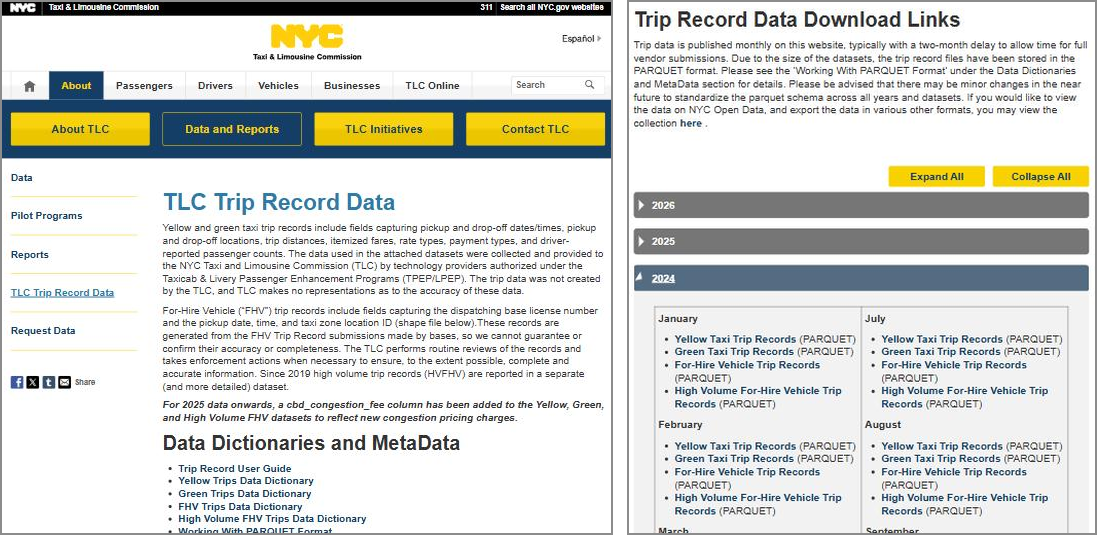
\includegraphics[width=\columnwidth]{figures/tlc_website.png}
\caption{The data source: the TLC Trip Record Data page on \texttt{nyc.gov}. Left:
description of the records and the data dictionaries. Right: monthly download links
(2024 expanded), one Parquet file per month and service type. Screenshots taken in
November 2026.}\label{fig:tlc}
\end{figure}

These questions are \emph{data parallel}: every record can be processed on its own and
the partial results combined by summation. They are therefore a natural fit for
MapReduce~\cite{dean2008mapreduce} and its in-memory successor
Spark~\cite{zaharia2012rdd,zaharia2016spark}, which split the input across machines
and run the same function on every split. What is less obvious is \emph{how much}
adding machines helps for data of this size, and when it stops helping.

\subsection{Problem statement and objectives}
Given the TLC yellow-taxi records, compute (i)~trip demand per zone and hour of day,
(ii)~the top-$N$ pickup$\rightarrow$drop-off routes, and (iii)~average fare and
credit-card tip rate per distance band; then measure how the run time changes when the
same work is spread over one, two, three or four machines. Our objectives are to:
\begin{enumerate}
  \item install and operate a Hadoop (HDFS, YARN, MapReduce) and Spark cluster in
        Docker containers, on one host and on a public cloud;
  \item implement the three analytics jobs as Python MapReduce programs;
  \item compare a single computer (one container) with multiple containers in
        run time, speedup and efficiency, and explain the differences.
\end{enumerate}

\subsection{Contributions}
\begin{itemize}
  \item A reproducible cluster: one Docker image and a Compose file for a master and
        1--4 workers with \emph{equal, capped} CPU and memory, plus scripts that run
        the full benchmark unattended.
  \item One Python implementation of each job, reused unchanged by Hadoop Streaming,
        Spark RDDs and a single-process baseline, with outputs cross-checked for
        equality.
  \item A strong- and weak-scaling study over six data sizes (1--24 months), 1--4
        workers and five execution engines on one host, repeated on Azure VMs:
        786 timed runs in total, plus a 48-run cache experiment.
\end{itemize}

\section{Project Activities}\label{sec:activities}

\subsection{Division of tasks}
\Cref{tab:team} lists who did what. Each member also wrote the report section on
their own part.

\begin{table}[t]
\centering
\caption{Team members and responsibilities}\label{tab:team}
\begin{tabularx}{\columnwidth}{@{}>{\raggedright\arraybackslash}p{0.22\columnwidth}>{\raggedright\arraybackslash}X@{}}
\toprule
Member & Responsibilities \\
\midrule
Chen Jinxian & Team lead; cluster infrastructure: Docker image, Compose file, Hadoop/YARN configuration, resource caps; report editing \\[2pt]
Yang Ye & Algorithms: mapper, reducer/combiner, PySpark jobs, serial baseline, correctness checks \\[2pt]
Gong Pengxiang & Data and benchmarking: data preparation, benchmark and cache-experiment scripts, figures \\[2pt]
Ma Jiajun & Cloud deployment on Azure, cloud measurements, demonstration video \\
\bottomrule
\end{tabularx}
\end{table}

\textbf{Timeline.} 23~Nov 2026: Docker image built and smoke test with two workers
passed. 24~Nov: data tiers prepared, Azure cluster deployed and the 225 cloud runs
completed; local benchmark started. 25~Nov: local benchmark (561 runs) and cache
experiment (48 runs) completed, figures and first report draft. December: report
revision and demonstration video.

\subsection{Installation process}
All software runs inside Docker containers~\cite{merkel2014docker}, so the host only needs Docker.
\begin{enumerate}
  \item \textbf{Host preparation.} Enable WSL\,2 on Windows~11 and install Docker
        Desktop with the WSL\,2 back end. Raise the memory available to the WSL\,2 VM
        in \texttt{.wslconfig} to 26\,GB, because the default limit (half of the
        host RAM) is too small for a master plus four 5\,GB workers.
  \item \textbf{Cluster image.} \texttt{cluster/Dockerfile} starts from Eclipse
        Temurin JDK\,11 on Ubuntu 22.04, adds Python~3, and unpacks Hadoop 3.4.1 and
        Spark 3.5.5 (pre-built for Hadoop~3). The Hadoop XML files and
        \texttt{spark-defaults.conf} are copied in, and all daemons run as an
        unprivileged \texttt{hadoop} user.
  \item \textbf{Roles.} The same image starts as \emph{master} (HDFS NameNode~\cite{shvachko2010hdfs}, YARN
        ResourceManager~\cite{vavilapalli2013yarn}, MapReduce JobHistory server) or \emph{worker} (DataNode and
        NodeManager), selected by \texttt{entrypoint.sh}.
  \item \textbf{Cluster start.} \texttt{scripts/cluster.sh up N} recreates the
        cluster with $N$ workers, waits until $N$ DataNodes and $N$ NodeManagers have
        registered, and uploads the Spark jars to HDFS once so that Spark jobs do not
        re-upload them on every submission.
  \item \textbf{Smoke test.} With two workers and tier S, all five engines and three
        jobs ran and their outputs matched. The web interfaces of HDFS (port 9870),
        YARN (8088) and the JobHistory server (19888) show the live nodes and every
        job; \cref{fig:yarn} shows the four-worker cluster.
\end{enumerate}

\begin{figure*}[t]
\centering
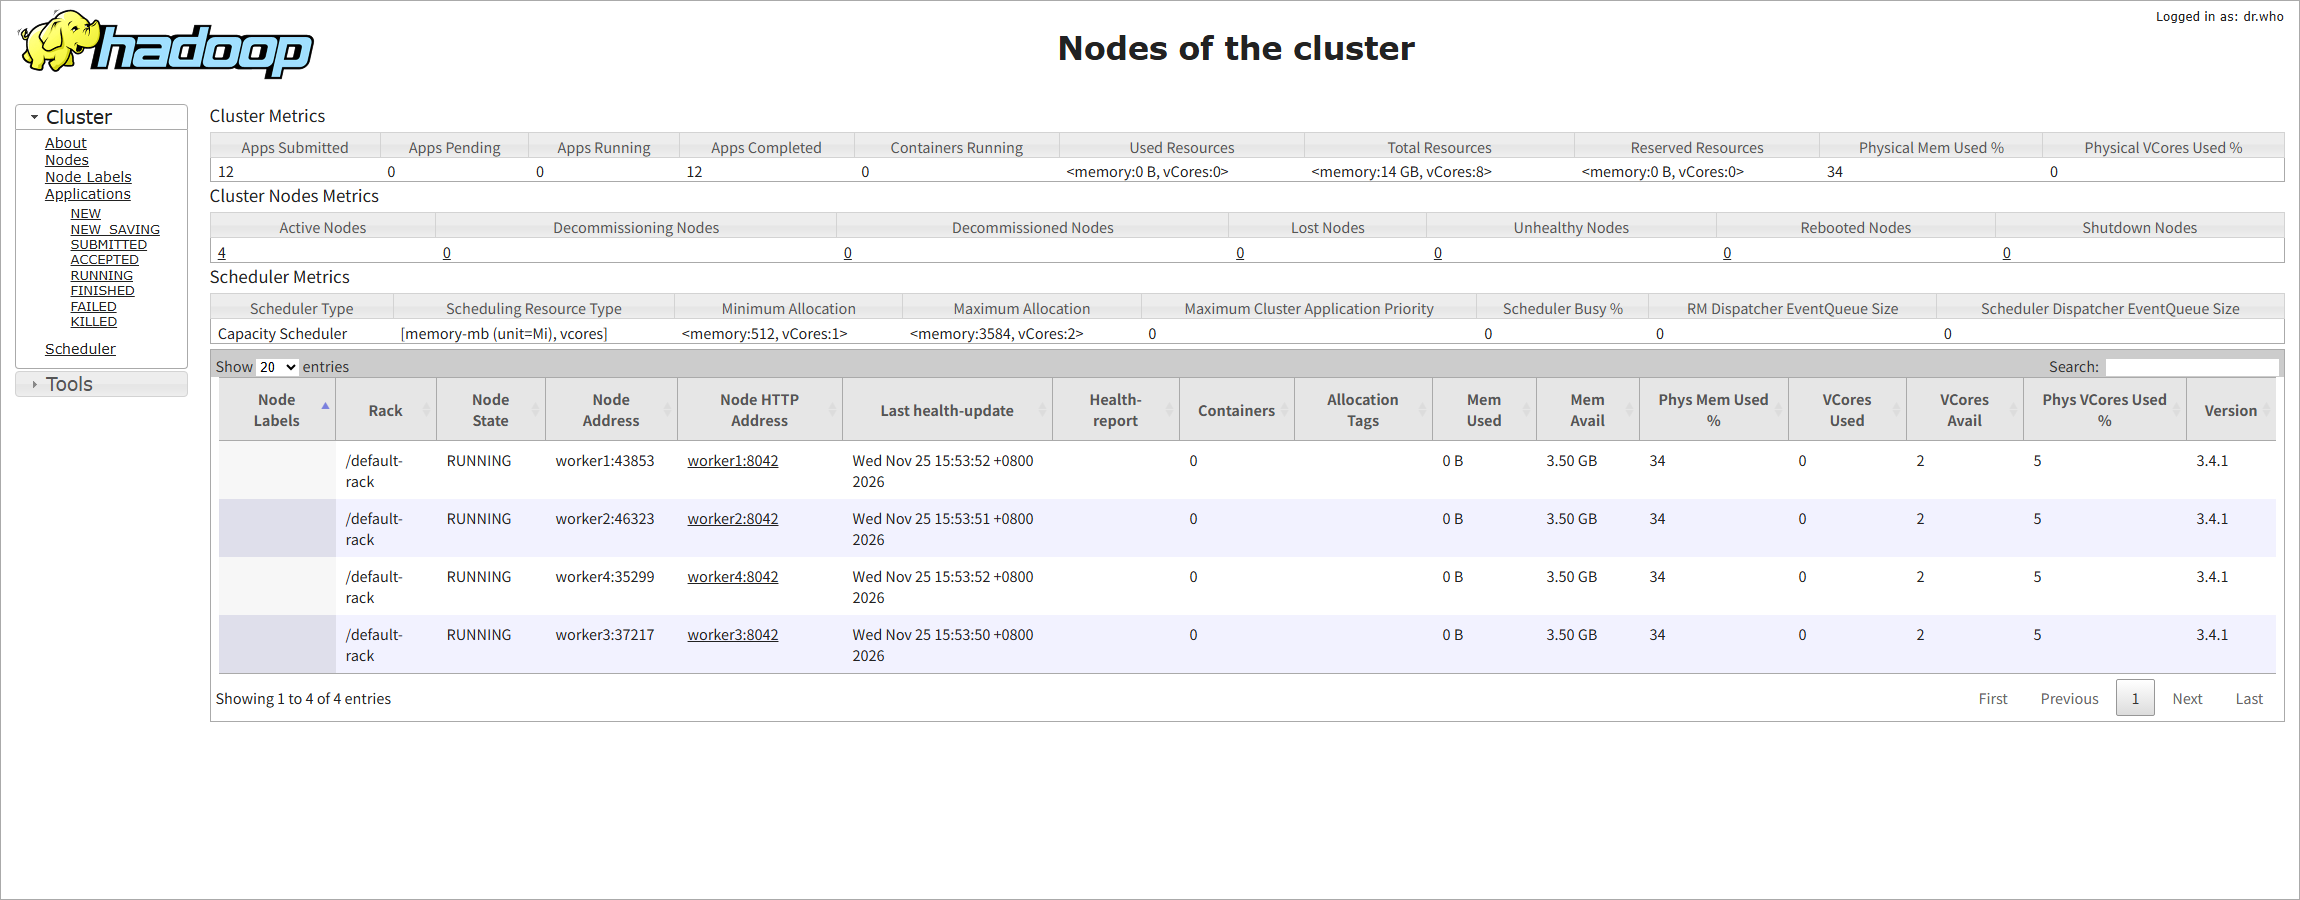
\includegraphics[width=\textwidth,trim=200 150 0 95,clip]{figures/yarn_nodes.png}
\caption{YARN ResourceManager web interface (port 8088) of the local cluster with four
workers: four active NodeManagers with 3.5\,GB and 2 vcores each (14\,GB and 8 vcores in
total), after the 12 jobs of the cache experiment on this cluster.}\label{fig:yarn}
\end{figure*}

\textbf{Problems and solutions.} (1)~Git Bash rewrites arguments such as
\texttt{/opt/scripts} into Windows paths before passing them to \texttt{docker}; the
scripts set \texttt{MSYS\_NO\_PATHCONV=1}. (2)~A separate \texttt{chown} layer in the
Dockerfile duplicated the Hadoop and Spark files and made the image 6.2\,GB; changing
ownership in the same layer as the extraction reduced it to 3.9\,GB. (3)~Without
explicit limits, one container could use all 20 host threads, so ``one worker'' was
not one machine; we cap CPU and memory per container and make YARN advertise the same
amounts. (4)~On Azure, a VM resolved its own name to an IPv6 link-local address that
the Hadoop daemons could not use; we pin all names to the private IPv4 addresses.
(5)~The full local sweep took many hours and was interrupted several times by restarts
of the WSL\,2 VM, Docker Desktop and Windows; \texttt{run\_benchmark.sh} therefore records every run and
skips completed ones when restarted.

\section{Algorithm and Implementation}\label{sec:algorithm}

\subsection{MapReduce formulation}
A MapReduce job applies a user \emph{map} function to every input record to produce
intermediate key--value pairs, groups the pairs by key (the \emph{shuffle}), and
applies a \emph{reduce} function to each group~\cite{dean2008mapreduce}. We chose a
single representation for all three jobs: the value is a numeric vector and the
reduce function is the element-wise sum. \Cref{tab:jobs} gives the keys and
vectors; averages and rankings are computed from the summed vectors afterwards, on
data that is at most a few thousand lines.

\begin{table}[t]
\centering
\caption{Keys and value vectors emitted by the mapper}\label{tab:jobs}
\begin{tabular*}{\columnwidth}{@{\extracolsep{\fill}}lll@{}}
\toprule
Job & Key & Value vector \\
\midrule
\texttt{demand} & pickup zone $|$ hour & $(1)$ \\
\texttt{routes} & pickup zone $|$ drop-off zone & $(1)$ \\
\texttt{fare}   & distance band & $(1,\ f,\ c,\ c\,f,\ c\,t)$ \\
\bottomrule
\multicolumn{3}{@{}p{\columnwidth}@{}}{\footnotesize $f$ = fare, $t$ = tip,
$c=1$ for credit-card trips (TLC records tips only for card payments), else $0$.}
\end{tabular*}
\end{table}

\begin{algorithm}[t]
\caption{Mapper, combiner/reducer and post-processing}\label{alg:mr}
\begin{algorithmic}[1]
\Procedure{Map}{line}
  \State $r \gets$ \Call{Parse}{line} \Comment{skip header and invalid rows}
  \If{$r \neq \bot$} \textbf{emit} $(\mathit{key}(r), \mathit{vec}(r))$ \EndIf
\EndProcedure
\Procedure{Reduce}{$k$, $[v_1,\dots,v_m]$} \Comment{also used as combiner}
  \State \textbf{emit} $(k, \sum_{i} v_i)$ \Comment{element-wise}
\EndProcedure
\Procedure{Post}{$\{(k, s_k)\}$}
  \State \texttt{routes}: sort by $s_k[0]$, keep top $N$
  \State \texttt{fare}: avg fare $= s[1]/s[0]$, tip rate $= s[4]/s[3]$
\EndProcedure
\end{algorithmic}
\end{algorithm}

\textbf{Combiner.} Because addition is associative and commutative, the reducer can
also run on each map task's output before the shuffle. For \texttt{fare} this
collapses millions of map outputs into a few lines per map task, so almost nothing
crosses the network; for \texttt{routes}, with $265^2$ possible keys, the reduction is
smaller. We measure both variants (\cref{sec:results}).

\textbf{Data cleaning.} \textsc{Parse} rejects rows with a malformed field, a zone
outside 1--265, a distance outside $(0,100)$ miles, a fare outside $(0,1000)$\,USD or a
negative tip (\cref{sec:data}).

\subsection{Execution engines}
\begin{itemize}
  \item \textbf{Hadoop Streaming}~\cite{hadoop_streaming,noll_streaming}.
        \texttt{mapper.py} and \texttt{reducer.py} read standard input and write
        tab-separated lines; Hadoop runs one mapper per
        128\,MB HDFS block and sorts map output by key before the reducers.
  \item \textbf{Spark RDD} (on YARN~\cite{spark_yarn}). \texttt{spark\_job.py --api rdd} imports the \emph{same}
        \texttt{parse} and \texttt{map\_record} functions; \texttt{flatMap} is the map
        phase and \texttt{reduceByKey} performs combining, shuffle and reduction.
        Intermediate data stays in memory instead of being written to local disk.
  \item \textbf{Spark DataFrame.} \texttt{--api df} expresses the same filters and
        aggregations in Spark SQL, so they are optimised by Catalyst and executed in
        the JVM without per-record Python calls.
  \item \textbf{Serial baseline.} \texttt{local\_baseline.py} applies the same
        functions in one Python process with an in-memory dictionary---the
        ``single computer'' reference.
\end{itemize}
Because all engines share one parser, any difference in run time comes from the
execution engine, not from the logic. \texttt{scripts/compare\_outputs.py} checks that
all engines give identical results; on the real data they do for every tier,
cluster size and environment (\cref{sec:results}).

\section{Deployment Environment}\label{sec:env}

\subsection{Local containerised cluster}
\Cref{fig:topology} shows the whole system. One master and up to four workers run as Docker
containers on a single host, connected by a user-defined bridge network in which each
container is reachable by its host name. The host and container specifications are
given in \cref{tab:env}.

\begin{figure}[t]
\centering
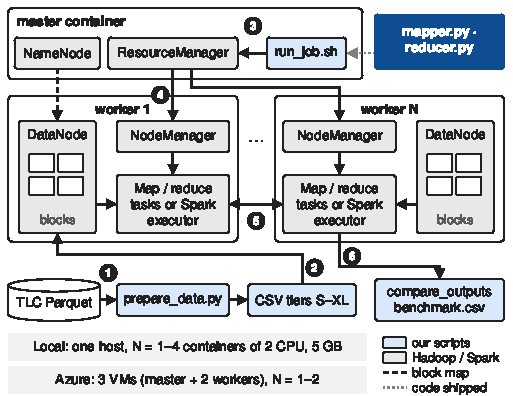
\includegraphics[width=\columnwidth]{figures/overview.pdf}
\caption{System overview. \textcircled{\scriptsize 1}~TLC Parquet files are cleaned
into CSV tiers and \textcircled{\scriptsize 2}~written to HDFS, whose 128\,MB blocks
are spread over the $N$ workers. \textcircled{\scriptsize 3}~\texttt{run\_job.sh}
submits a job to the ResourceManager, which \textcircled{\scriptsize 4}~starts map and
reduce tasks or a Spark executor next to the blocks;
\textcircled{\scriptsize 5}~intermediate pairs are shuffled between workers and
\textcircled{\scriptsize 6}~the merged output is checked and timed. The same image and
the same mapper/reducer code (the only part every engine shares) run on one host and on
Azure. The JobHistory server and the Spark driver also run on the master.}\label{fig:topology}
\end{figure}

\begin{table}[t]
\centering
\caption{Hardware and software environment}\label{tab:env}
\begin{tabularx}{\columnwidth}{@{}lX@{}}
\toprule
Host CPU & Intel Core i5-13600KF (6P+8E cores, 20 threads) \\
Host memory / disk & 32\,GB / 2\,TB NVMe SSD \\
Host OS & Windows 11, Docker Desktop 4.100 (WSL\,2) \\
\midrule
Worker container & 2 CPUs, 5\,GB RAM (\texttt{cpus}, \texttt{mem\_limit}) \\
YARN per worker & 2 vcores, 3584\,MB for containers \\
Master container & 2 CPUs, 4\,GB RAM \\
\midrule
Software & Ubuntu 22.04, OpenJDK 11, Python 3.10 \\
         & Hadoop 3.4.1, Spark 3.5.5 on YARN \\
HDFS & block 128\,MB, replication 1 \\
\bottomrule
\end{tabularx}
\end{table}

\textbf{Fair comparison on one host.} Without limits, a single container may use all
20 host threads, and ``one node'' would not be one node. Every worker is therefore
capped at the same 2~CPUs and 5\,GB, and YARN advertises exactly those resources.
Adding a worker thus adds a fixed amount of compute. Spark uses one executor with two
cores per worker; Hadoop schedules map and reduce containers of 1\,GB each. HDFS
replication is 1, so adding workers spreads the input rather than copying it.

\subsection{Public-cloud cluster}
To measure a real multi-machine cluster we used Microsoft Azure (Azure for Students
subscription). The subscription allows at most six vCPUs per region and four per VM
family, and restricts deployments to five Asian regions; Korea Central was the
allowed region offering Dv4 sizes. We therefore deployed three Ubuntu 22.04 VMs in one
virtual network: a master (\texttt{Standard\_D2\_v4}, Intel Xeon Platinum 8370C) and
two identical workers (\texttt{Standard\_D2s\_v4}, Xeon Platinum 8272CL), each with
2~vCPUs, 8\,GB RAM and a StandardSSD disk. On these sizes the two vCPUs are the two
hyper-threads of one physical core. Network security rules admit SSH only from our
address; all cluster traffic stays inside the virtual network.

The VMs run the \emph{same} Docker image as the local cluster (Docker 29.1), built
once on the master and copied to the workers. Containers use the host network, so the
node names are the VM names; they are pinned to the private IPv4 addresses in
\texttt{/etc/hosts}, because Azure's Ubuntu image resolves a VM's own name to an IPv6
link-local address that Hadoop clients cannot use. Each VM is one node: no container
caps are needed, and YARN advertises the same 2~vcores and 3584\,MB as locally. The
scripts in \texttt{cloud/} create the VMs (Azure CLI), deploy the image and data,
start 1 or 2 workers, and delete everything afterwards. The cloud cluster cost about
US\$0.38 per hour (three VMs, public IPs and disks); the whole cloud study, about
11~hours including deployment, cost about US\$4 (estimated from list prices) of the
student credit. The VMs were deleted afterwards.

\section{Data Sources}\label{sec:data}

We use the TLC Yellow Taxi Trip Records~\cite{tlc_data} for January 2023 to December
2024. Each month is published as an Apache Parquet file with one row per trip and
about twenty columns, together with a lookup table that maps the 265 taxi-zone IDs to
zone and borough names. \texttt{scripts/prepare\_data.py} downloads the files and
converts each month to a header-less CSV with the eight columns the jobs need;
\cref{tab:schema} shows them with the first trip of January 2024. CSV is used because
Hadoop Streaming feeds mappers with lines of text.

\begin{table}[t]
\centering
\caption{Columns used, with the first trip of January 2024 as an example}\label{tab:schema}
\setlength{\tabcolsep}{4pt}
\begin{tabularx}{\columnwidth}{@{}>{\ttfamily}ll>{\raggedright\arraybackslash}X@{}}
\toprule
\normalfont Column (TLC name) & Example & Use \\
\midrule
tpep\_pickup\_datetime & 2024-01-01 00:57:55 & hour (\texttt{demand}) \\
PULocationID & 186 (Penn Station) & pickup zone \\
DOLocationID & 79 (East Village) & drop-off zone \\
trip\_distance & 1.72 (miles) & band; cleaning \\
fare\_amount & 17.70 (US\$) & mean fare \\
tip\_amount & 0.00 (US\$) & tip rate \\
total\_amount & 22.70 (US\$) & not used \\
payment\_type & 2 (cash) & 1 = card: tip known \\
\bottomrule
\end{tabularx}
\end{table}

\begin{figure*}[t]
\centering
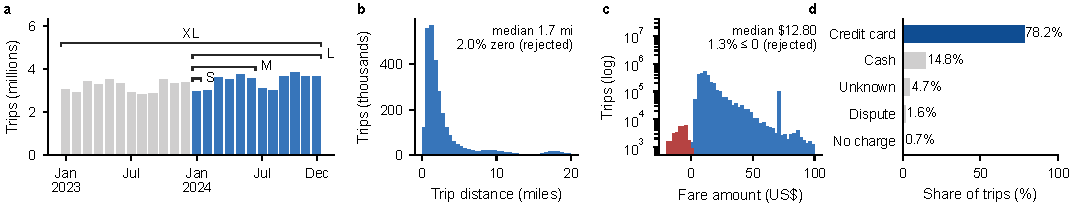
\includegraphics[width=\textwidth]{figures/data_overview.pdf}
\caption{What the input looks like. (a)~Yellow-taxi trips per month, January 2023 to
December 2024 (Parquet row counts), and the nested tiers S, M, L and XL.
(b)--(d)~January 2024: (b)~trip distance up to 20~miles, (c)~fare amount (log scale;
red: zero or negative fares, which are rejected), (d)~payment types.}\label{fig:data}
\end{figure*}

\Cref{fig:data} shows what the records look like. Demand is steady at 2.8--3.8~million
trips per month (lowest in August 2023, highest in October 2024), so every month adds a
similar amount of work. Most trips are short: the median distance is 1.7~miles and the
median fare US\$12.80. The spike at US\$70 is the flat fare between JFK Airport and
Manhattan (3.3\% of the trips). 78\% of the trips are paid by credit card, the only
payment type for which tips are recorded; 15\% are paid in cash.

To study how scaling depends on data size, the months are grouped into nested tiers
(\cref{tab:tiers}). Every monthly file is 140--180\,MiB, i.e.\ two 128\,MB HDFS
blocks, so Hadoop starts about two map tasks per month: 2 for tier S but 48 for
tier XL. Tiers S, M, L and XL are used for strong scaling; W3 and W9 complete the
weak-scaling series of three months per worker (W3, M, W9, L for 1--4 workers).

\begin{table}[t]
\centering
\caption{Dataset tiers (valid = rows passing the cleaning rules)}\label{tab:tiers}
\begin{tabular*}{\columnwidth}{@{\extracolsep{\fill}}llrrr@{}}
\toprule
Tier & Period & Rows & Valid & CSV size \\
\midrule
S  & Jan 2024 (1 mo.)       & \num{2964624}  & 96.8\% & 142\,MiB \\
W3 & Jan--Mar 2024 (3 mo.)  & \num{9554778}  & 96.4\% & 457\,MiB \\
M  & Jan--Jun 2024 (6 mo.)  & \num{20332093} & 96.7\% & 974\,MiB \\
W9 & Jan--Sep 2024 (9 mo.)  & \num{30021209} & 96.6\% & 1.40\,GiB \\
L  & 2024 (12 mo.)          & \num{41169720} & 96.4\% & 1.93\,GiB \\
XL & 2023--2024 (24 mo.)    & \num{79479946} & 96.7\% & 3.72\,GiB \\
\bottomrule
\end{tabular*}
\end{table}

\textbf{Data quality.} The raw records contain zero or negative distances and fares
(2.0\% and 1.3\% of the trips in January 2024), implausible values and missing payment
types. Records failing the rules in \cref{sec:algorithm} are dropped: \num{1464575} of
\num{41169720} rows (3.6\%) in tier L and \num{2587058} (3.3\%) in tier XL. Tips are
analysed only for credit-card trips, because cash tips are not recorded.

\section{Results}\label{sec:results}

\noindent\textbf{Main findings at a glance.}
\begin{itemize}
  \item \emph{Small data:} on one month the clusters are 4--6$\times$ slower than a
        single Python process, because start-up costs 13--23\,s per job.
  \item \emph{Large data:} on two years four workers are up to 4.0$\times$ faster than
        one; Spark DataFrame is the fastest engine, up to 5.1$\times$ faster than serial.
  \item \emph{Single host vs.\ cloud:} two Azure VMs scale more regularly than two
        containers on one host, but each VM is slower.
\end{itemize}

\subsection{Method}
For each cluster size $N\in\{1,2,3,4\}$ the cluster is rebuilt from scratch, a data
tier is loaded into HDFS, and every combination of job and engine is run three times
(twice on tier XL) by \texttt{scripts/run\_benchmark.sh}; the serial baseline runs
once per tier in a single process. Runs of one configuration follow each other, so
repetitions 2 and 3 start with a warm operating-system cache. We report the mean
wall-clock time from job submission to completion, which includes start-up and
scheduling overhead, and its standard deviation. In total we recorded 561 runs on the
local cluster and 225 on Azure, all successful. With $T_1$ the time of the same engine
on one worker and $T_\text{serial}$ the time of the single-process baseline, we use
\begin{equation}
S_\text{rel}(N)=\frac{T_1}{T_N},\qquad E(N)=\frac{S_\text{rel}(N)}{N},\qquad
S_\text{abs}(N)=\frac{T_\text{serial}}{T_N}.
\end{equation}
To estimate the non-parallel fraction we use the Karp--Flatt
metric~\cite{karp1990measuring}, $e=\frac{1/S_\text{rel}-1/N}{1-1/N}$, and interpret
it with Amdahl's law~\cite{amdahl1967validity}. For weak scaling, each worker receives
three months of data (tiers W3, M, W9, L for $N=1..4$) and the efficiency is
$T(1,\text{W3})/T(N,3N\text{ months})$.

\subsection{Analytics output}
\Cref{fig:run} shows one real run: the \texttt{routes} job on tier L with four
workers. Hadoop splits the 24 monthly blocks into 24 map tasks, 20 of them on the
worker that stores the block; the combiner shrinks 39.7~million map outputs to
\num{537298} records before the shuffle, and the job writes \num{50127} routes in
60.8\,s. \Cref{fig:analytics} shows the answers to the three questions for the full year 2024
(tier L, \num{39705145} valid trips). Demand peaks at 18:00 with 2.82~million trips
over the year and is lowest at 04:00 (0.23~million); the busiest zone--hour pair is
Midtown Center at 18:00 (\num{164630} pickups). The busiest zones differ in
\emph{when} they are busy: Midtown peaks in the evening rush hour, the Upper East Side
during the day, and JFK Airport is the only one with substantial traffic after
midnight. The five most frequent routes all start and end in the Upper East Side or
Midtown, i.e.\ short trips inside Manhattan. Average fares grow with distance, while
the credit-card tip rate falls from 28.8\% of the fare for trips under one mile to
17.1\% for trips over 20~miles.

\begin{figure}[t]
\begin{lstlisting}[style=terminal]
$ docker exec master /opt/scripts/run_job.sh mr routes L 4
INFO mapreduce.JobSubmitter: number of splits:24
INFO impl.YarnClientImpl: Submitted application
     application_1795551341851_0087
INFO mapreduce.Job:  map 0% reduce 0%
INFO mapreduce.Job:  map 50% reduce 0%
INFO mapreduce.Job:  map 100% reduce 45%
INFO mapreduce.Job:  map 100% reduce 100%
INFO mapreduce.Job: Job job_1795551341851_0087 completed
     successfully
  Launched map tasks=24       Data-local map tasks=20
  Map input records=41169720
  Map output records=39705145
  Combine output records=537298
  Reduce shuffle bytes=6656616
  Reduce output records=50127
SECONDS 60.84
$ sort -k2 -nr outputs/mr-routes-L.tsv | head -3
237|236    275994
236|237    237909
237|237    184456
\end{lstlisting}
\caption{A real run (abridged; timestamps removed): \texttt{routes} on tier L with
four workers, Hadoop progress and job counters, the run time printed by
\texttt{run\_job.sh}, and the three most frequent routes in the output
(zone 237 = Upper East Side South, 236 = Upper East Side North).}\label{fig:run}
\end{figure}

\begin{figure*}[t]
\centering
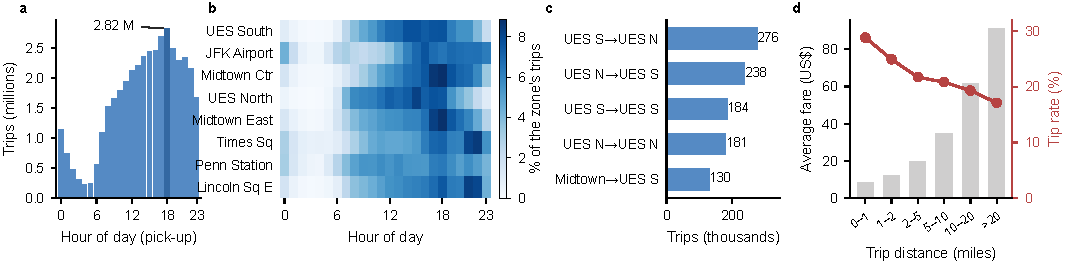
\includegraphics[width=\textwidth]{figures/analytics_L.pdf}
\caption{What the three jobs found in the 39.7~million valid trips of 2024 (tier L,
identical for all engines). (a)~\texttt{demand}: trips per hour of day, peak at 18:00.
(b)~\texttt{demand}: hourly profile of the eight busiest pick-up zones, each row
normalised to the zone's total (UES = Upper East Side). (c)~\texttt{routes}: the five
most frequent pick-up$\rightarrow$drop-off zone pairs. (d)~\texttt{fare}: average fare
(bars) and credit-card tip rate (line) per distance band.}\label{fig:analytics}
\end{figure*}

\subsection{Run time and speedup on the local cluster}
\Cref{fig:scaling} shows the \texttt{routes} job on every tier; the other two jobs
behave in the same way, and \cref{tab:summary} lists all jobs for tier L.

\begin{figure*}[t]
\centering
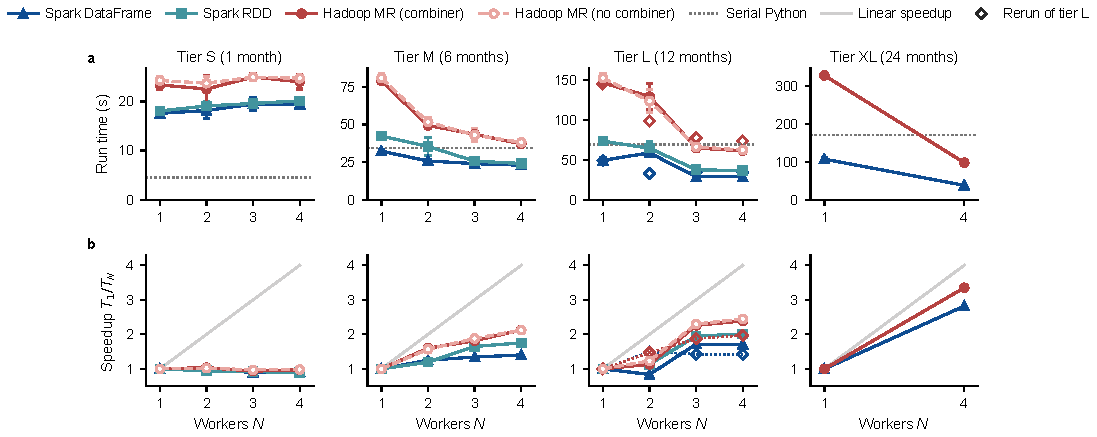
\includegraphics[width=\textwidth]{figures/scaling_routes.pdf}
\caption{Strong scaling of the \texttt{routes} job on the local cluster, one column per
data tier. (a)~Mean run time with one standard deviation; dotted: serial baseline.
(b)~Relative speedup $T_1/T_N$; grey: linear speedup. Open diamonds: the warm runs of
the later cache experiment on tier L (\cref{tab:cache}), which do not show the dip at
$N=2$. Tier XL was run with 1 and 4 workers only.}\label{fig:scaling}
\end{figure*}

\begin{table*}[t]
\centering
\caption{Tier L (12 months, 1.93\,GiB) on the local cluster: mean run time (s) per
number of workers, and relative speedup, efficiency, speedup over the serial baseline
and Karp--Flatt serial fraction at $N=4$. Bold: fastest engine of each job. Standard
deviations are in
\texttt{results/summary.csv}.}\label{tab:summary}
\begin{tabular*}{\textwidth}{@{\extracolsep{\fill}}llrrrrrrrr@{}}
\toprule
Job & Engine & $T_1$ & $T_2$ & $T_3$ & $T_4$ & $S_\text{rel}(4)$ & $E(4)$ & $S_\text{abs}(4)$ & $e(4)$ \\
\midrule
\inputrows{generated/summary_table.tex}
\bottomrule
\end{tabular*}
\end{table*}

\textbf{Small data (tier S).} The serial baseline needs 4.3--4.5\,s per job, whereas
every cluster configuration needs 17--23\,s with Spark and 22--27\,s with MapReduce,
independently of $N$ ($S_\text{rel}\approx1$). The run time is almost entirely fixed
cost: submitting the application, starting the YARN application master and the
executor or task JVMs, and writing the output.

\textbf{Medium and large data.} From tier M on, adding workers reduces the run time.
At $N=4$, MapReduce reaches $S_\text{rel}=2.0$--$2.2$ on tier M and 2.4--2.8 on tier
L; Spark RDD 1.7--1.8 and 2.0--2.4; Spark DataFrame 1.4--1.6 and 1.7--1.9. On tier XL,
MapReduce speeds up by 3.35--3.97 from one to four workers ($E=0.84$--$0.99$) and the
DataFrame engine by 2.25--3.05. In absolute terms Spark DataFrame is always fastest:
on tier L with four workers it needs 29\,s per job, 2.2--2.4$\times$ faster than the
serial baseline, and on tier XL 38--39\,s, 3.6--5.1$\times$ faster than the serial
baseline (139--195\,s). On tier L, Hadoop MapReduce on one worker is 2.1--2.6$\times$
slower than the serial baseline and only matches it with three or four workers on tier L
($S_\text{abs}(4)=1.03$--$1.13$); on tier XL it is 1.4--1.75$\times$ faster.

\textbf{The two-worker anomaly.} On tier L the step from one to two workers gives
almost no gain (MapReduce $S_\text{rel}(2)=1.08$--$1.34$; Spark DataFrame 0.84--1.18,
i.e.\ \texttt{routes} became slower), MapReduce run times at $N=2$ vary strongly
(standard deviation up to 23\,s), and the step from two to three workers is then
\emph{superlinear} (MapReduce 1.8--2.1$\times$ for 1.5$\times$ the workers). The same
step on tier M is regular ($S_\text{rel}(2)=1.5$--$1.6$ for MapReduce). A controlled
rerun did not reproduce the anomaly (\cref{sec:discussion}).

\textbf{Weak scaling.} With three months of data per worker
(\cref{fig:weak}) the efficiency at four workers is 0.79 for Spark DataFrame, 0.75 for
Spark RDD and 0.70 (0.67 without combiner) for MapReduce, averaged over the three jobs.

\begin{figure}[t]
\centering
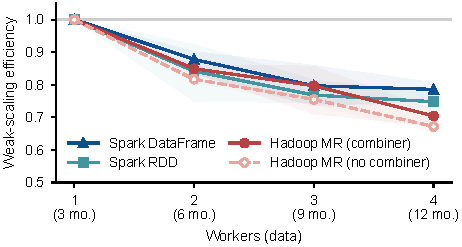
\includegraphics[width=\columnwidth]{figures/weak_scaling.pdf}
\caption{Weak-scaling efficiency $T(1,\text{W3})/T(N,3N\text{ months})$ with three
months of data per worker: mean of the three jobs (lines) and their range
(shading).}\label{fig:weak}
\end{figure}

\subsection{Effect of the combiner}
\Cref{fig:combcloud}a shows the data shuffled from map to reduce tasks on tier L,
from the MapReduce job counters. All three jobs emit the same 39.7~million map output
records; the combiner shrinks the shuffle by a factor of 72 for \texttt{routes}, 309
for \texttt{demand} and about \num{100000} for \texttt{fare}, where the records
collapse to 216 per run (1.1\,GiB to 12\,KiB). The run-time effect depends on the
job: on one worker \texttt{fare} is 24\% faster with the combiner (169 vs.\ 223\,s)
and 20\% faster at $N=4$, whereas \texttt{demand} and \texttt{routes} change by less
than the run-to-run variation (\cref{tab:summary}). On Azure with two workers the
combiner saves 29\% for \texttt{fare} (236 vs.\ 332\,s) and 7--10\% for the other jobs.

\begin{figure}[t]
\centering
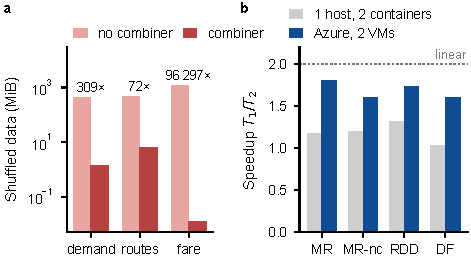
\includegraphics[width=\columnwidth]{figures/combiner_cloud.pdf}
\caption{(a)~Data shuffled per MapReduce job on tier L without and with the combiner
(log scale; labels: reduction factor). (b)~Speedup from one to two workers on tier L,
run times summed over the three jobs: two containers on one host vs.\ two Azure VMs
(MR-nc: MapReduce without combiner).}\label{fig:combcloud}
\end{figure}

\subsection{Public cloud}
\Cref{fig:combcloud}b compares the same software and configuration on the local
containers and on the Azure VMs. On one worker, Azure is 2.0$\times$ slower for the
serial baseline (388 vs.\ 197\,s for the three jobs) and 2.5--3.3$\times$ slower for
the cluster engines (e.g.\ Spark DataFrame 449 vs.\ 154\,s, MapReduce 1221 vs.\
463\,s). On the other hand the Azure cluster scales better from one to two workers:
on tier L the summed speedup is 1.60--1.80 on Azure (efficiency 0.80--0.90) against
1.03--1.31 locally. On tier M both environments behave similarly (Azure MapReduce
1.68--2.03, Spark 1.37--1.65; local MapReduce 1.52--1.64, Spark 1.19--1.40). On tier S
the cloud cluster shows no speedup either ($S_\text{rel}=0.97$--$1.12$), with a fixed
cost of about 40\,s per job for Spark and 55\,s for MapReduce.

\subsection{Correctness}
For every tier and cluster size, the outputs of Hadoop MapReduce (with and without
combiner), Spark RDD and Spark DataFrame agree with the serial baseline
(\texttt{compare\_outputs.py}; money sums agree to within the 0.01 rounding of the
printed values). The outputs computed on Azure are identical to the local ones.

\section{Discussion}\label{sec:discussion}

\subsection{When does distribution pay off?}
Every cluster run pays a fixed cost that does not depend on the input: about 13--18\,s
for Spark and 18--23\,s for MapReduce on the local cluster (the tier~S time minus the
serial time), and about twice as much on the slower cloud VMs. On one month of data
this cost is three to five times the whole serial computation, so a cluster is
pointless at that size. Spark DataFrame on one worker breaks even with the serial
baseline at about six months of data (tier M, 1\,GB) and is 1.2--1.4$\times$ faster at
twelve months. MapReduce needs three to four workers to match the serial program on 2\,GB and wins clearly only
on 3.7\,GB (tier XL). Note that one worker has two CPUs while the serial program uses
one, so this comparison even favours the cluster.

The weak-scaling efficiency of 0.67--0.79 at four workers shows the same effect from
the other side: when the data grow with the cluster, the run time grows only slowly,
mainly because the fixed cost is paid once per job rather than once per worker.

\subsection{Scalability and its limits}
\textbf{Amdahl's law.} The Karp--Flatt estimate on tier L at $N=4$ is
$e=0.15$--$0.22$ for MapReduce, 0.23--0.33 for Spark RDD and 0.37--0.44 for Spark
DataFrame (\cref{tab:summary}). These values roughly agree with a simple model in
which the fixed cost is the serial part: for Spark DataFrame, about 15\,s of fixed cost
out of $T_1\approx50$\,s is a serial fraction of about 0.3, which by Amdahl's law
bounds the speedup to about~3.3 however many workers are added; for MapReduce, about
20\,s out of 150\,s gives 0.13. The fastest engine therefore scales
\emph{worst}: its parallel part is so short that the constant start-up dominates. On
tier XL the parallel part is larger and $e$ drops to 0.10--0.26 for Spark DataFrame and
below 0.07 for MapReduce. Relative speedup alone would make MapReduce look like the
better system; the absolute times show the opposite.

\textbf{Task granularity.} Tier L has 24 HDFS blocks and hence 24 map tasks. YARN
schedules by memory, so each worker runs three 1\,GB containers, one of which hosts
the MapReduce application master. With three workers 8 maps run at once (exactly three
waves); with four workers 11 run at once, and the third wave contains only two tasks.
This explains why MapReduce gains only 4--15\% from the fourth worker on tier L but
3.35--3.97$\times$ from one to four workers on tier XL (48 tasks).

\begin{table}[t]
\centering
\caption{Cache experiment, \texttt{routes} on tier L: mean run time (s) after dropping
the page cache (cold) and directly afterwards (warm), largest disk read in a warm run,
and CPU time withheld by the 2-CPU cap per worker and second (3 pairs per cell)}\label{tab:cache}
\setlength{\tabcolsep}{2.5pt}
\begin{tabular*}{\columnwidth}{@{\extracolsep{\fill}}rrrrrrrrr@{}}
\toprule
 & Data/wkr & \multicolumn{2}{c}{MapReduce} & \multicolumn{2}{c}{Spark DF} & Warm read & \multicolumn{2}{c}{Throttled} \\
\cmidrule(lr){3-4}\cmidrule(lr){5-6}\cmidrule(l){8-9}
$N$ & (GiB) & cold & warm & cold & warm & (MiB) & MR & DF \\
\midrule
\inputrows{generated/cache_table.tex}
\bottomrule
\end{tabular*}
\end{table}

\textbf{The two-worker anomaly.} The poor result at $N=2$ on tier L
(\cref{sec:results}) is specific to one tier and one environment. Our first
hypothesis was the page cache: the 5\,GB limit of a container also counts the cached
HDFS blocks, so with one or two workers holding 1--2\,GB each, blocks might be re-read
from the shared virtual disk. We tested it with a further 48 runs
(\cref{tab:cache}): \texttt{routes} on tier L with $N=1$--4, MapReduce and Spark
DataFrame, three pairs each, where the page cache of the Docker VM is dropped before
the \emph{cold} run and the \emph{warm} run follows directly. For each worker we read
the cgroup counters for bytes read from disk, refaulted cache pages and throttled CPU
time. The hypothesis is \emph{refuted}: even with all 2.3\,GiB on one worker, warm
runs read at most 3\,MiB from disk, no page was refaulted and no container reached its
memory limit, and cold runs, which read the whole input from disk, differ from warm
runs by less than 5\,s. Moreover, the anomaly did not reproduce: at $N=2$ the rerun gives
$S_\text{rel}(2)\approx1.5$ for both engines, on a smooth curve between $N=1$ and
$N=3$. In the main benchmark all $N=2$ runs on tier L fell into one hour of the night
(01:30--02:30) and the configurations ran in a fixed order, so we attribute the anomaly
to a transient disturbance on the host during that hour, which we cannot identify
after the fact. The rerun also shows the size of session-to-session variation on a
shared host: at $N=1$ it matches the main benchmark within 3\%, but at $N=3$--4 its
warm runs are 20\% slower, so MapReduce reaches only $S_\text{rel}(4)\approx2.0$ instead of 2.4.
Speedups on tier L therefore carry an uncertainty of this order.

The throttling counters support the task-granularity argument. A MapReduce worker runs
three 1\,GB containers, each a JVM plus a Python process, on a 2-CPU quota: the cap
withholds 0.7 CPU-seconds per second at $N=1$, where one container is the application
master, and 1.4--1.7 at $N\ge2$, where a worker runs three map tasks. Spark runs one
2-core executor per worker and is throttled by only 0.2. MapReduce is thus CPU-bound
and oversubscribed. Finally, the \texttt{cpus} limit caps CPU time but does not pin
containers to cores, so on the hybrid i5-13600KF a worker may run on a performance core,
an efficiency core or a hyper-thread of a busy core.

\subsection{Effect of the combiner}
The combiner reduces the shuffle by two to five orders of magnitude
(\cref{fig:combcloud}a), but saves time only when the shuffle is large compared with
the rest of the job. On \texttt{fare} the uncombined shuffle (1.1\,GiB) is 2.5--2.8
times that of \texttt{demand} or \texttt{routes}, and the combiner saves up to 24\%
locally and 29\% on Azure. For the other two jobs, 400--450\,MiB are shuffled without measurable
cost on one host, where the ``network'' is a virtual bridge in memory, but the combiner
saves 7--10\% on Azure, where the data cross a real network. On a larger cluster with
slower links we expect the benefit to grow.

\subsection{Hadoop MapReduce vs.\ Spark}
On one worker and tier L, Spark RDD is 2.0--2.1$\times$ faster than MapReduce and Spark
DataFrame 3.0--3.1$\times$ faster, although all three run the same algorithm. MapReduce
starts a new JVM for every task, writes and sorts all map output on local disk before
the reduce phase, and, with Streaming, passes every record as text through a pipe to a
Python process and back. Spark reuses one executor per worker for all tasks and
aggregates in an in-memory hash table~\cite{zaharia2012rdd}. Spark RDD still calls the
Python \texttt{parse} and \texttt{map\_record} functions once per record and moves data
between the JVM and Python workers; the DataFrame version runs entirely in the JVM.
The 1.5$\times$ difference between Spark RDD and DataFrame is therefore the cost of
executing user code in Python, and the remaining 2$\times$ between MapReduce and Spark
RDD is the cost of the disk-based MapReduce execution model.

\subsection{Single host vs.\ public cloud}
The local machine is faster per worker: the serial program runs 2.0$\times$ faster on
one i5-13600KF core than on one Azure vCPU, and the engines 2.5--3.3$\times$ faster.
Two Azure vCPUs are the two hyper-threads of one older server core, whereas a local
worker usually gets two separate modern cores. The cloud, however, scales more
regularly, because each worker there owns its disk, memory and network interface. The
single-host cluster is cheap and convenient for development, but adding containers on
one host adds CPU quota, not independent hardware, and its speedup measurements can be
distorted by shared resources. The cloud cluster cost about US\$4 for all experiments;
for the same money the local machine was faster, but it cannot grow beyond one host.

\subsection{Lessons learned}
(1)~\emph{Measure the fixed cost first.} One run on one month told us more about when
a cluster pays off than any estimate: below about 1\,GB the start-up cost dominates.
(2)~\emph{Containers are not machines.} Without caps one container used the whole host;
even with caps they share a disk, and our measurements varied by 20\% between
sessions, so multi-machine claims need real machines. (3)~\emph{Write the logic once,
check every output.} One shared parser and an automatic output comparison made every
speed comparison fair. (4)~\emph{Automate and make runs resumable.} The 10-hour sweep
was interrupted several times; recording each run let us resume instead of restarting.
(5)~\emph{Test an explanation before writing it.} Our first explanation of the
two-worker anomaly, the page cache, was wrong.

\subsection{Threats to validity}
(i)~All local workers share one host, disk and memory bus (see above). (ii)~Only two
cloud workers were possible within the student subscription's limit of six vCPUs per
region, and the cloud master uses a different CPU model than the workers.
(iii)~Repetitions were consecutive and the configurations ran in a fixed order, so a
disturbance of the host affects all repetitions of one configuration, as at $N=2$ on
tier L; a rerun in another session differed by up to 20\%. A warm page cache, in
contrast, changes run times by at most 5\,s (\cref{tab:cache}). (iv)~Apart from the
cache experiment we measured wall-clock time only, and even there not network
traffic or per-core CPU utilisation. (v)~The input is CSV converted from Parquet,
which favours line-based Hadoop Streaming; Spark could read Parquet directly.

\section{Conclusion}\label{sec:conclusion}
We built a containerised Hadoop and Spark cluster, ran it on one host with up to four
workers and on three Azure VMs, and used it to analyse 79.5~million NYC taxi trips
with three data-parallel jobs written once in Python. All engines produced identical
results. Distribution pays off only above roughly 1\,GB of input: on one month of data
the fixed start-up cost of 13--23\,s exceeds the 4.5\,s serial run. On 3.7\,GB, four
workers run 3.3--4.0$\times$ faster than one with MapReduce and 2.2--3.1$\times$ with
Spark DataFrame, and Spark DataFrame is 3.6--5.1$\times$ faster than the serial
program. The fastest engine scales worst because its fixed cost becomes the serial
fraction, so absolute times must be reported along with speedups. The combiner
reduced the shuffle by up to five orders of magnitude but saved time mainly for the
shuffle-heavy \texttt{fare} job and on the real cloud network. Two VMs scaled more
regularly than two containers on one host. A poor two-worker result on one host was
not caused by the page cache, as a controlled experiment showed, and did not reproduce
in a rerun; it shows that measurements on a shared host vary by about 20\% between
sessions.

\textbf{Future work.} (i)~Randomise and interleave the run order and repeat every
configuration in several sessions, so that host disturbances average out;
(ii)~repeat the cloud study with three or four workers in a region with free quota;
(iii)~deploy the same image on Kubernetes; (iv)~read Parquet directly in Spark.

\medskip
\noindent\textbf{Source code and video.} \TODO{Repository URL} \quad
\TODO{Demonstration video URL}


\bibliographystyle{IEEEtran}
\bibliography{refs}

\appendices
% Listings are read directly from the files that were run, so the report
% always shows the current code.
\section{Source Code}\label{app:code}
The MapReduce code shared by all engines is listed below. The PySpark jobs
(\texttt{code/spark\_job.py}), the serial baseline (\texttt{code/local\_baseline.py}),
which calls the same mapper and reducer functions in one process, the cluster definition (\texttt{cluster/}), the
benchmark and plotting scripts (\texttt{scripts/}) and the cloud deployment scripts
(\texttt{cloud/}) are in the repository.

\subsection{Mapper (\texttt{code/mapper.py})}
\lstinputlisting[language=Python]{\coderoot/mapper.py}

\subsection{Reducer and combiner (\texttt{code/reducer.py})}
\lstinputlisting[language=Python]{\coderoot/reducer.py}

\end{document}
